\documentclass{article}

\usepackage[utf8]{inputenc}
\usepackage[german]{babel}
\usepackage[
    a4paper, top=2.5cm, bottom=2.5cm, left=2.5cm, right=2.5cm, marginparwidth=1.75cm
]{geometry}
\usepackage{amsmath}
\usepackage{amsfonts}
\usepackage{enumitem}
\usepackage[
    colorlinks=true, 
    citecolor=black,
    filecolor=black,
    linkcolor=black,
    urlcolor=blue
]{hyperref}
\usepackage{graphicx}
\usepackage{multirow}
\usepackage{amssymb}
\usepackage{float}
\usepackage{siunitx} \sisetup{locale = DE, uncertainty-mode = separate}
\usepackage{pdfpages}
\usepackage{multirow}
\usepackage[
    tocskip=0.1\baselineskip, skip=0.7\baselineskip, parfill
]{parskip}
\usepackage{listings}
\usepackage{fancyhdr}
\usepackage{xcolor}

% Kopf- und Fußzeile
\pagestyle{fancy}
\fancyhf{}
%Kopfzeile mittig mit Kaptilname
\fancyhead[C]{\nouppercase{\leftmark}}
%Fußzeile links bzw. innen
\fancyfoot[L]{\versuchsname}
%Fußzeile mittig (Seitennummer)
\fancyfoot[R]{\thepage}
\renewcommand{\footrulewidth}{0.35pt}

% Hilfs-Commands für Gleichungen
\newcommand{\widespace}{\enspace}
\newcommand{\wideeq}{\widespace = \widespace}
\newcommand{\wideneq}{\widespace \neq \widespace}
\newcommand{\wideapprox}{\widespace \approx \widespace}
\newcommand{\wideleq}{\widespace \leq \widespace}
\newcommand{\widegeq}{\widespace \geq \widespace}
\newcommand{\widele}{\widespace \le \widespace}
\newcommand{\widege}{\widespace \ge \widespace}
\newcommand{\wideiff}{\widespace \iff \widespace}
\newcommand{\wideimplies}{\widespace \implies \widespace}
\newcommand{\pd}[2]{
    \frac{\partial #1}{\partial #2}
}

% Markieren von verwendetem Code
\definecolor{codebg}{RGB}{230, 240, 255}
\newcommand{\coderef}[1]{%
    \text{\footnotesize \colorbox{codebg}{\texttt{#1()}}}%
}

% Formatieren von Code im Anhang
\definecolor{codegreen}{rgb}{0,0.6,0}
\definecolor{codegray}{rgb}{0.5,0.5,0.5}
\definecolor{codepurple}{rgb}{0.58,0,0.82}
\definecolor{backcolour}{rgb}{0.95,0.95,0.92}
\lstdefinestyle{mystyle}{
    backgroundcolor=\color{backcolour},   
    commentstyle=\color{codegreen},
    keywordstyle=\color{magenta},
    numberstyle=\tiny\color{codegray},
    stringstyle=\color{codepurple},
    basicstyle=\ttfamily\footnotesize,
    breakatwhitespace=false,         
    breaklines=true,                 
    captionpos=b,                    
    keepspaces=true,                 
    numbers=left,                    
    numbersep=5pt,                  
    showspaces=false,                
    showstringspaces=false,
    showtabs=false,
    tabsize=4
}

\lstset{style=mystyle}

% Formatierung von Absätzen
\renewcommand{\baselinestretch}{1.2}

\allowdisplaybreaks

% Allgemeine Infos
\newcommand{\versuchsname}{
    NMR-A - Kernspinresonanz
}
\newcommand{\githuburl}{
    \url{https://github.com/WeinSim/P3B}
}

% Titel und Autor
\title{\versuchsname}
\author{Simon Weinzierl, Yannic Werner}

\begin{document}

\maketitle

\begin{center}
    Physikalisches Fortgeschrittenenpraktikum P3B
    nach der Studienordnung für Studienbeginn bis WS 2022/23
\end{center}

\vspace*{6cm}

\begin{center}
    \footnotesize
    Alle Teile dieses Dokuments (Vorbereitung, Protokoll, Auswertung) wurden
    von beiden Teilnehmern in gleichen Teilen und ohne fremde Hilfe bearbeitet.
    Sofern fremde Quellen verwendet wurden, sind diese angegeben.

    Der \LaTeX-Code ist auf GitHub unter \githuburl verfügbar.
    
    © Alle Rechte vorbehalten.
\end{center}

 % LMU-Siegel
\AddToShipoutPicture*{
    \put(315,0){
        \parbox[b][5cm]{5cm}{
            
\includegraphics[width=10cm]{Abbildungen/Siegel_LMU.pdf}
        }
    }
}

\newpage

% Inhaltsverzeichnis
\tableofcontents

\newpage

% Literatur
\bibliographystyle{alpha}
\bibliography{literatur}

\newpage


\section{Vobereitung}

\subsection{Physikalischer Hintergrund}

\subsubsection{Magnetisches Moment}

\cite{chemie.de}

Das magnetische Moment ist in der Physik ein Maß für die Stärke eines Magnetfeldes. Das magentische Moment, auch magnetischse Dipolmoment genannt, ist somit neben dem elektrischen Moment eine weitere Größe in der Stromverteilung der Physik.

Möchte man das magnetische Moment mathematisch ausdrücken, so lässt sich folgenden Formel aufstellen:

\[
    \vec{m} \wideeq I \, \vec{A}
    \wideeq \frac{1}{2} \sum_i q_i \, \vec{r}_i \times \vec{v}_i
    \wideeq \frac{1}{2} \int \mathrm{d}^3 r \,
    \left[ \vec r \times \vec j (\vec r) \right]
\]

Aus der allgemeinen Formel (Produkt aus Stromstärke und Flächenvektor), lässt sich also die Formel zur exakten Berechnung aufstellen.

Möchte man nun das magentische Moment in verschiedenen Situationen überprüfen, so kann man die aufgestelle Formel noch weiter präzisieren. Hierfür werden im Folgenden drei konkrete Fäller genauer betrachtet:

\begin{enumerate}
    \item \textit{Ebene Leiteschleife.} \quad Da für eine geschlossene Leiterschleife
    
    \[
        \vec{j} \, \mathrm{d}^3 r \wideeq I \, \mathrm{d} \vec{r}
    \]
    
    gilt, folgt für das magenetische Moment:

    \[
        \vec{m}
        \wideeq \frac{I}{2} \int_C \left( \vec{r} \times \mathrm{d} \vec{r} \right)
        \wideeq I \cdot \vec{A}
        \wideeq I A \vec{e}
    \]

    Wie ersichtlich, genügt es also, den Zusammenhang aus Stromfläche und Querschnittsfläche mit dem Einheitsvektor zu multiplizieren.

    \item \textit{Stromdurchflossene lange Spule.} \quad
    Hierbei spiel die Windungszahl der Spule eine zentrale Rolle:

    Die Formel des magentischen Moments lässt sich in diesem Fall gsnz einfach erweitern: die Windungszahl wird einfach mit dem Produkt aus Stromstärke und Fläche multipliziert. Somit erhält man:

    \[
        m \wideeq nIA
    \]

    Sofern man nun Kenntnis über das magnetische Moment des Dipols hat, lässt sich das auf den Körper einwirkende Magentfeld mittels

    \[
        \vec{M} \wideeq \vec{m} \times \vec{B}
    \]

    berechnen. Hierbei muss man jedoch aufpassen, da alle Größen vektorielle Größen sind, also die Richtung ein zentrale Rolle spielt!

    \item \textit{Teilchen.} \quad
    Für ein Teilchen lässt sich das magenetische Moment $\mu$
    \[
        \vec{\mu} \wideeq g \, \frac{q}{2m} \, \vec{S}
    \]

     mit $g$ als gyromanischen Faktor und $\vec{S}$ als Spin, welcher erst in Kapitel 1.1.2 genauer betrachtet wird.

    Betrachtet man ausschließlich ein Elektron, so lässt sich die Formel umstellen zu:

    \[
        \mu_B \wideeq \frac{e\hbar}{2m_e}
    \]

    Folgend nun eine Herleitung des Ausdrucks für das magentische Moment eines Teilches aus der allgemeinen Definition für eine Schleife:

    \[
        \vec{\mu}
        \wideeq \frac 1 2 \int \mathrm{d}^3 r \,
        \left[ \vec r \times \vec j (\vec r) \right]
    \]

    mit

    \[
        \vec j (\vec r, t) \wideeq q \vec v (t)
        \delta^{(3)} \left( \vec r - \vec r (t) \right)
    \]

    Darus folgt: 

    \[
        \vec{\mu}(t) \wideeq \frac{q}{2}\,\vec{r}(t)\times \vec{v}(t)
    \]

    Mittelt man dies nun für eine gebundene, stationäre Bewegung über die Zeit:

    \[
        \langle \vec{\mu} \rangle
        \wideeq \frac 1 T \int_0^T \vec{\mu}(t) \, \mathrm{d}t
        \wideeq \frac{q}{2T} \int_0^T \vec{r}(t) \times \vec{v}(t) \, \mathrm{d}t
        \wideeq \frac{q}{2m} \, \vec{L}
    \]

    Speziell in der NMR-Spektroskopie, also für Atomkerne, schreibt man die Formel für das magentische Moment als:

    \[
        \vec{\mu} \wideeq \frac{q}{e} \gamma \vec{S}
    \]

    mit $\frac{q}{e}$ als Elementraladung und $\gamma$ als gyromagentisches Verhältnis, definiert als:

    \[
        \gamma \wideeq \frac{g\mu_{B}}{\hbar}
    \]
    
\end{enumerate}

\subsubsection{Spin}

\cite{rptu}

\cite{chemie.de_2}

Der Spin eines Teilchens ist wie die Masse oder die Ladung eine fundamentale
Eigenschaft. Er hat eine große Relevanz für die Struktur von Atomen und Molekülen.
Zudem ist der Spin der Grund für die Entstehung von Magnetfeldern,
beziehungsweise die Basis von Magnetismus.
Nun gibt es zwei Möglichkeiten, wie man ein Teilchen betrachtet:

\begin{enumerate}
    \item Teilchen als Kreisel, die sich drehen: hierbei betrachtet man die Teilchen als System, welches sich um seine eigene Achse dreht. Somit kann jedem Teilchen ein Drehimpuls zugeordnet werden. Diese Vorstellung hilf der Veranschaulichung, entspricht jedoch nicht der Realität.
    \item Teilchen als winzige Magnete: da der Spin ein Magnetfeld zur Folge hat, kann man sich die Teilchen modellhaft als winizige Stabmagneten vortsellen. Dabei können sich die Teilchen aber nicht in jede Richtung drehen wie ein Stabmagnet, da die Ausrichtung der quantenmechanischen Momente gequantelt ist. Elektronen können hier zum Beispiel lediglich die zwei Zustände $\left| \uparrow \right>$ (``Spin up'') und $\left| \downarrow \right>$ (``Spin down'') einnehmen.

\end{enumerate}

Da wir nun eine korrekte Vorstellung über den Spin haben, wollen wir  im Folgenden noch einige Eigenschaften des Spins genauer betrachten:
\begin{enumerate}
    \item Spinquantenzahl und Spineigenzustand:
        \begin{itemize}
            \item Die Eigenzustände und -werte lassen sich analog zum Drehimpuls bestimmten. Hierfür muss folgende Eigenwertgleichung gelöst werden:
            \[
                S^2 \Psi \wideeq s (s + 1) \hbar^2 \Psi \to S_z \Psi = s_z \hbar \Psi
            \]
            mit $\Psi$ als Zustandsvektor.
            \item $S^2$ ist dabei definiert als
            \[
                S^2 = S_X^2+S_Y^2+S_Z^2
            \]
            mit $S_{z}$ als Spinoperatoren und $s_{z}$ als Spinquntenzahlen.
            \item Die möglichen $s_z$-Werte sind gegen durch
            \[
                -s,-s+1-...,s-1,s
            \]
            Also sind für jedes Spinkomponente ($s_x$, $s_y$, $s_z$) $2s+1$ verschiedene Werte möglich.
        \end{itemize}
    \item Spin als Erhlatungsgröße
        \begin{itemize}
            \item Spinquantenzahl eines Elementarteilchens ist unveränderlich; Spinausrichtung jedoch nicht
            \item Gesamtspin ist keine Erhaltungsgröße; aber Gesamtdrehimpuls (werden Reaktionen in der Atomphysik betrachtet, so ist die Summe der Eigendrehimpulswerte vor und nach der Reaktion die gleiche)
        \end{itemize}
    \item Spin und magentisches Moment
        \begin{itemize}
            \item Spin eines Elementarteilchens kann über das magentische Moment gemessen werden
            \item Über magnetisches Moment tritt Spin in Wechselwirkung mit magnetischen Feldern (die magnetische Energie eines Teilchens ist von dessen Orientierung relativ zum Magnetfeld abhängig)
            \item Atom: Wecheslwirkungen zwischen Elektronen und Atomkern und zwischen Elektronen untereinander (Ausnutzen in Kernspinresonanz)
        \end{itemize}  
    \end{enumerate}

\subsubsection{Spinpräzession}

\cite{sdw}

\cite{tech}

Da nun der Spin und seine Eigenschaften verstanden wurden, wollen wir im Folgenden die Spinpräzession genauer betrachten.

Spinpräzession beschreibt hierbei die Präzessionsbewegung des Spins eines Elementarteilchens (Elektron) in einem magnetischen Feld. Dabei hat der Spin nur zwei Möglichkeiten für dessen Wert, gegeben durch die magentischen Quantenzahle $m_s=\pm\frac{1}{2}$. Folglich nimmt der Spindrehimpuls die Werte $s_z=\pm\frac{1}{2}\hbar$ an.

Dieses Phänomen spielt eine zentrale Rolle beim Aufbau der Atom (Larmor-Präzession). Folgende Skizze soll die Präzession des Elektronenspins um die Quantisierungsachse $z$ veranschaulichen:

\begin{figure}[H]
    \centering
    \includegraphics[width=0.4\linewidth]{Abbildungen/Spinpräzession.jpeg}
    \caption{Präzession des Elektronenspins um die Quantisierungsachse $z$}
\end{figure}

\subsubsection{Erwartungswert des Spins}

\cite{dm}

\cite{tss}

Der Erwartungswert beschreibt den Wert, welcher der Mittelwert über viele identische Messungen wäre. Dabei muss der Erwartungswert selbst jedoch kein möglicher Messwert sein. Für jede Observable ist der Erartungwert gegen durch: 
\[
    \langle A \rangle = \text{Tr}(\rho A)
\]
wobei $\rho$ gegeben ist als $\rho = | \psi \rangle \langle \psi |$.

Möchte man nun den Erwartungswert in der Dynmaik betrachten, so gilt im Magentgelf $B$ mit dem Hamiltonoperator $H=-\gamma B \cdot S$:
\[
    \frac{d}{dt} \langle S \rangle \wideeq \gamma \langle S \rangle \times B
\]
Diese Gleichung beschreibt eine Präzessionsbewegung des Erwartungswert des Spins um die Magnetfeldachse.

Jedoch muss man für eine Messung entlang einer Einheitsrichtung folgendes beachten, bevor man die Berechnung durchführt bei Spins ($\frac{1}{2}$):

\[
    \langle S_{\hat{n}} \rangle \wideeq \frac{\hbar}{2} r\cdot \hat{n}
\]

\subsubsection{Kernmagneton $\mu_n$}

Das Kernmagneton $\mu_n$ wird in der Kern- und Teilchenphysik als Einheit für magnetische Momente verwendet. Dabei ist das Kernmagneton definiert als: 
    \[
        \mu_n \wideeq \frac{e\hbar}{2m_p} \wideeq \frac{m}{m_p}\mu_B
    \]
Wie ersichtlich betrachtet man hier nun Protonen und keine Elektronen ($m_p$).

Man verwendet das Kernmagneton also analog zum Bohrschen Magenton für Elektronen. Durch den enormen Masseunterschied von Elektronen und Kern/Protonen sind deren magentische Momente viel kleiner als die von Elektronen. 

\subsubsection{$g$-Faktor}

\cite{Dem}

Zwischen dem Bahndrehmoment $\mathbf l$ und dem magnetischen Moment $\boldsymbol \mu_l$
eines Elektrons besteht der Zusammenhang
\[
    \boldsymbol \mu_l
    \wideeq - \frac{\mu_B}{\hbar} \mathbf l
    \wideeq - \frac{e}{2 m_e} \mathbf l,
\]
welcher dem klassisch erwarteten Wert eines Teilchens mit Ladung $-e$, Masse $m_e$
und Bahndrehimpuls $\mathbf l$ entspricht.

Zwischen dem Spindrehmoment $\mathbf s$ und dem dadurch erzeugten magnetischen Moment
$\boldsymbol \mu_s$ besteht ein angloger Zusammenhang, jedoch mit einer
unterschiedlichen Proportionalitätskonstante:
\[
    \boldsymbol \mu_s
    \wideeq - g_s \frac{\mu_B}{\hbar} \mathbf l
    \wideeq - g_s \frac{e}{2 m_e} \mathbf l
\]
Hier ist $g_s \approx 2$ der $g$-Faktor des Elektrons. Der Spindrehimpuls
trägt also ungefähr doppelt so viel zum gesamten magnetischen Moment
$\boldsymbol \mu_j = \boldsymbol \mu_l + \boldsymbol \mu_s$ bei wie der Bahndrehimpuls.

Befindet sich ein Atom in einem äußeren elektrischen Feld $\mathbf B$,
dann gilt für den Erwartungswert $\langle \mu_j \rangle$
des magnetischen Moments:
\[
    \langle \mu_j \rangle
    \wideeq - g_j \frac{\mu_B}{\hbar} | \boldsymbol \mu_j |
    \wideeq - g_j \frac{e}{2 m_e} | \boldsymbol \mu_j |
\]
Hier wurde der $g$-Faktor entsprechend angepasst:
\[
    g_j \wideeq 1 + \frac{j (j + 1) + s (s + 1) - l (l + 1)}{2 j (j + 1)}
\]
Daraus folgt, dass sich unterschiedliche Energieniveaus unter dem Einfluss
eines (schwachen) externen magnetischen Feldes unterschiedlich stark aufspalten.


\subsubsection{Auswahlregeln}

\cite{Dem}

Nicht alle Übergänge zwischen zwei Energiezuständen in einem Atom können durch
elektromagnetische Strahlung angeregt werden. Neben der Energieerhaltung
gibt es weitere Regeln für Übergänge, die aufgrund von Symmetrien oder anderen
Erhaltungsgrößen zustande kommen.

Für optische Dipolübergänge lauten die Auswahlregeln:
\begin{align*}
    \Delta m &\wideeq \begin{cases}
        \pm 1 \quad &\text{für zirkular polarisiertes Licht} \\
        0 \quad & \text{für linear polarisiertes Licht}
    \end{cases} \\
    \Delta l &\wideeq \pm 1 \\
    \Delta S &\wideeq 0 \\
    \Delta J &\wideeq 0, \pm 1 \quad \text{aber } J = 0 \not \to J = 0
\end{align*}

Für optische Quadrupolübergänge gelten andere Auswahlregeln, beispielsweise
gilt hier $\Delta l = 0, \pm 2$.


\subsubsection{Grundiwssen des P2-Versuchs OSZ (s. Durchführung)}

    \begin{enumerate}
        \item Teilversuch 1: Belastungsabhängigkeit zweier Spannungsquellen
            \begin{itemize}
                \item Jede Spannungsquelle hat einen Innenwiderstand. Dadurch sinkt die Klemmspannung mit zunehmendem Laststrom
                \item Galvanische Zelle belasten und dann Strom und Spannung in mehreren Stufen messen
                \item Zuerst und am Ende der Leerlaufspannung bestimmen
            \end{itemize}
        \item Teilversuch 2: Bestätigung des Ohmschen Gesetzes
            \begin{itemize}
                 \item FÜr Ohmsche Leiter gilt $I \alpha U$
                \item Widerstand ist konstant
            \end{itemize}
        \item Teilversuch 3: Spannungsabfall und Potentiometer
            \begin{itemize}
                \item Nach dem Ohmschen Gesetz fällt an einem Leiterstück die Spannung proportional zur Länge ab
                \item Potentiometer dienen als Spannungsleiter
            \end{itemize}
        \item Teilversuch 4: Spannungsmessung durch Komponenten
            \begin{itemize}
                \item Kompensationsmessung verhindert Belastung der Spannungsquelle
                \item Leerlaufspannung exakt messen
            \end{itemize}
        \item Zusammenfassung und Zusammenhänge mit NMR
            \begin{itemize}
                \item Zeigen Zusammenhang zwischen Spannung, Strom, Widerstand und Energierehaltung von elektrischen Stromkreisen
                \item NMR-Geräte arbeiten mir komplexen elektrischen Schaltungen (Spulen erzeugen das B-Feld)
                \item Ohmsches Gesetz und Sapannungsabfälle sind entscheidend für die Signalstärke und Rauschunterdrückung
                \item Das Potentiometer/Spannungsteiler-Prinzip steckt in der Feinabstimmung von NMR-Geräten
                \item Die Kompensationsmessung ist direkt verwandt mit der empfindlichen Spannungsmessung
                \item Die Kirchhoffschen Sätze sind die Basis der Schaltungsanalyse in der NMR-Elektronik
            \end{itemize}
    \end{enumerate}


\newpage

\section{Veruschsablaufplan}

\subsection{Benötigte Materialien}
    \begin{enumerate}[label=\arabic*.]
        \item NMR-Betriebsgerät
        \item NMR-Versorgungseinheit
        \item U-Magnetkern mit Aufsatz
        \item Spuel 10A, 480 Windungen
        \item DC-Spannungsquelle 0...16V, 0...5A
        \item Analog-Oszilloskop HM 507
        \item BNC-Kabel 1m
        \item geschirmtes BNC-Kabel
        \item Sicherheitsverbundungskabel, 50cm, rot
        \item Sicherheitsverbindungskabel, 100cm, rot
        \item SIcherheitsverbindungskabel, 100cm, blau
        \item Universal-Physik-Messgerät
        \item Combi B-Sensor S
        \item Verlängerungskabel, 15-polig
    \end{enumerate}

\newpage


\subsection{Teilversuch 1: NMR an flüssigen und festen Proben mit Protonen}
\begin{enumerate}[label = (\Roman*)]
    \item Ziel: Bestimmen der Kerspinresonanzfrequenzen einzelner Proben
    
    \item Versuchsmethode: Demonstrieren der Kernspinresonant einer Glyzerin-, sowie einer Wasser- und einer Polystyrolprobe
    
    \item Versuchsskizze:
    
        \begin{figure}[H]
        \centering
        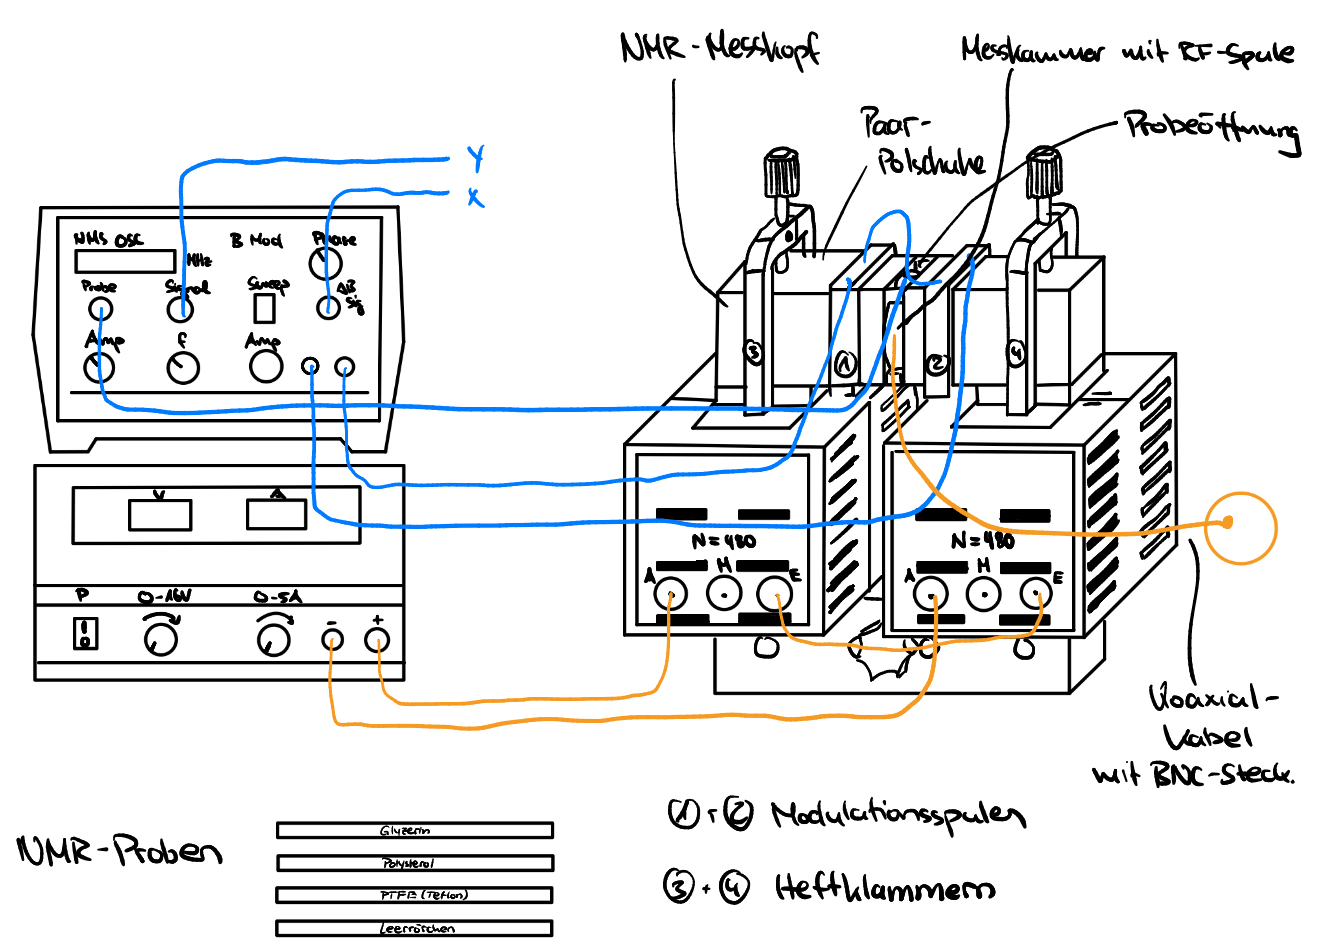
\includegraphics[width=0.7\linewidth]{Abbildungen/TV1-5.jpeg}
        \caption{Versuchsskizze Teilversuch 1}
        \end{figure}

    \item Planung der Durchführung
        \begin{itemize}
            \item Geräteeinstellung: Lissajous-Figuren sollen am Oszilloskop dargestellt werden. Einstellen einer Frequenz von circa 19MHz
            \item Einsetzen der Glyzerin-Probe so, dass sie sich in der Mitte der Messkammer befindet
            \item Strom durch die beiden 10A Spulen so lange erhöhren, bis das MNR-A Signal auf dem Oszilloskopbild erkennbar wird (wenn kein Signal findbar, dann ist die Amplitude am Oszillator ungünstig eingestellt) 
            \item Je kleiner Amplitude, umso ausgeprägter ist Resonanzsignal, aber auch Rauschen
            \item Resonanzkurve ausdrucken und mit den notwendigen Daten beschriften
        \end{itemize}

    \item Vorüberlegungen zur Durchführung \& Auswertung
        \begin{itemize}
            \item Bis TV5 soll das B-Feld nicht mehr verändert werden! Optimieren des Bildes auf dem Oszilloskop mit verschiedenen Parametern
            \item Mittels Drehknopf Phase kann das positive Signal mit dem negativen Signal zur Deckung gebracht werden
        \end{itemize}
\end{enumerate}

\newpage

\subsection{Teilversuch 2: NMR an einer festen Probe mit Fluorkernen}
\begin{enumerate}[label = (\Roman*)]
    \item Ziel: Vergleich der Messung einer festen Probe mit Fluorkernen mit den Ergebnissen aus Teilversuch 1
    
    \item Versuchsmethode: Messen der Resonanzkurve des Spins des Fluorkerns
    
    \item Versuchsskizze:
    
        \begin{figure}[H]
        \centering
        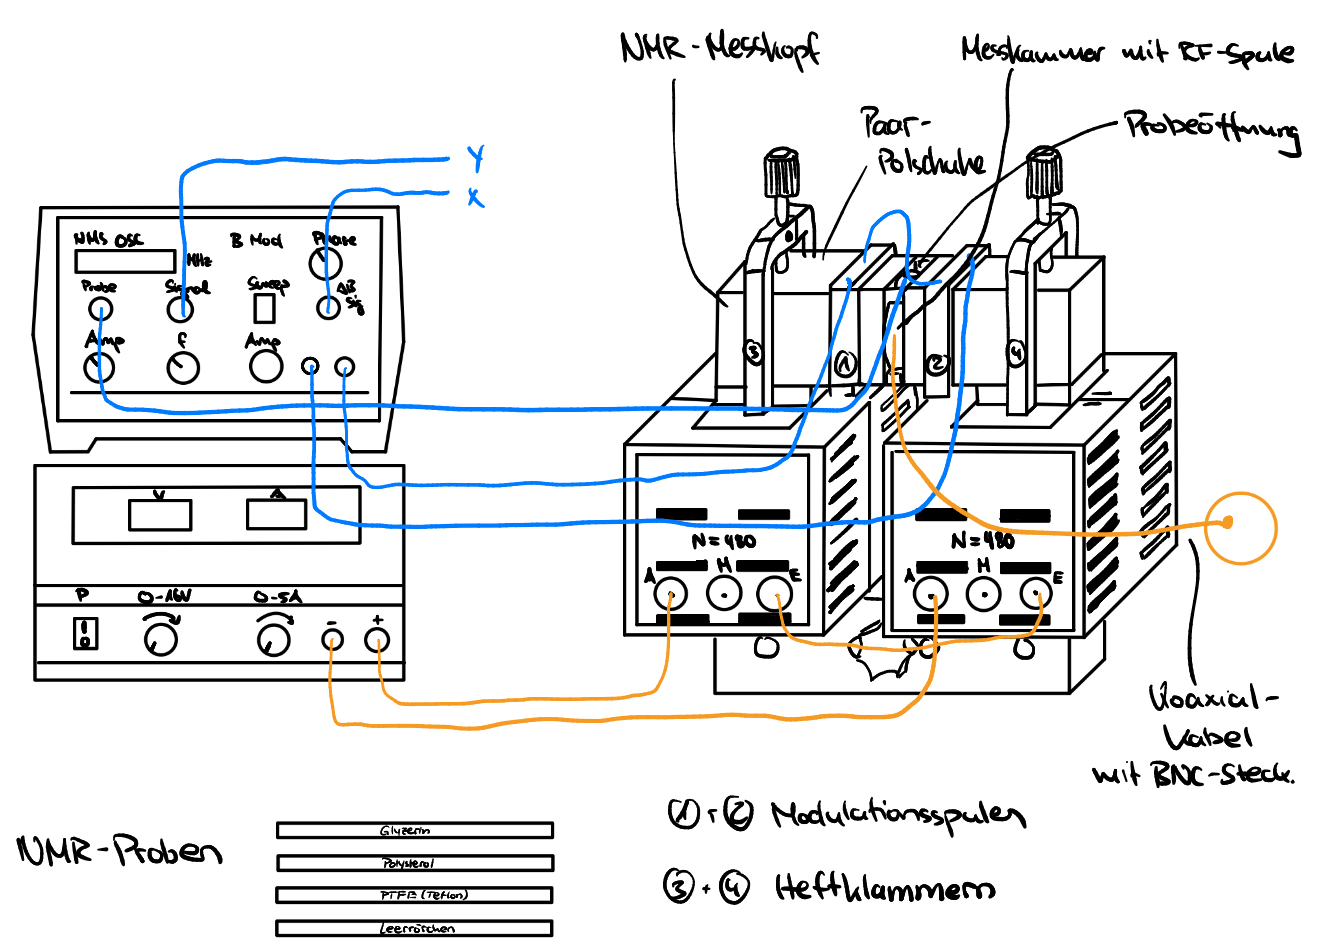
\includegraphics[width=0.7\linewidth]{Abbildungen/TV1-5.jpeg}
        \caption{Versuchsskizze Teilversuch 2}
        \end{figure}

    \item Planung der Durchführung
        \begin{itemize}
           \item Geräteeinstellung: Lissajous-Figuren sollen am Oszilloskop dargestellt werden. Einstellen einer Frequenz von circa 19MHz
            \item Einsetzen des Fluorkerns so, dass sie sich in der Mitte der Messkammer befindet
            \item Strom durch die beiden 10A Spulen so lange erhöhren, bis das MNR-A Signal auf dem Oszilloskopbild erkennbar wird (wenn kein Signal findbar, dann ist die Amplitude am Oszillator ungünstig eingestellt) 
            \item Je kleiner Amplitude, umso ausgeprägter ist Resonanzsignal, aber auch Rauschen
            \item Resonanzkurve ausdrucken und mit den notwendigen Daten beschriften
        \end{itemize}

    \item Vorüberlegungen zur Durchführung \& Auswertung
        \begin{itemize}
            \item Bis TV5 soll das B-Feld nicht mehr verändert werden! Optimieren des Bildes auf dem Oszilloskop mit verschiedenen Parametern
            \item Mittels Drehknopf Phase kann das positive Signal mit dem negativen Signal zur Deckung gebracht werden
        \end{itemize}
        
\end{enumerate}


\newpage

\subsection{Teilversuch 3: Bestimmung der Resonanzbreite}
\begin{enumerate}[label = (\Roman*)]
    \item Ziel: Bestimmen der Resonanzbreite
    
    \item Versuchsmethode: Bestimmen der Halbwertsbreite der Resonanzlinie von verschiedenen Kernen
    
    \item Versuchsskizze:
    
        \begin{figure}[H]
        \centering
        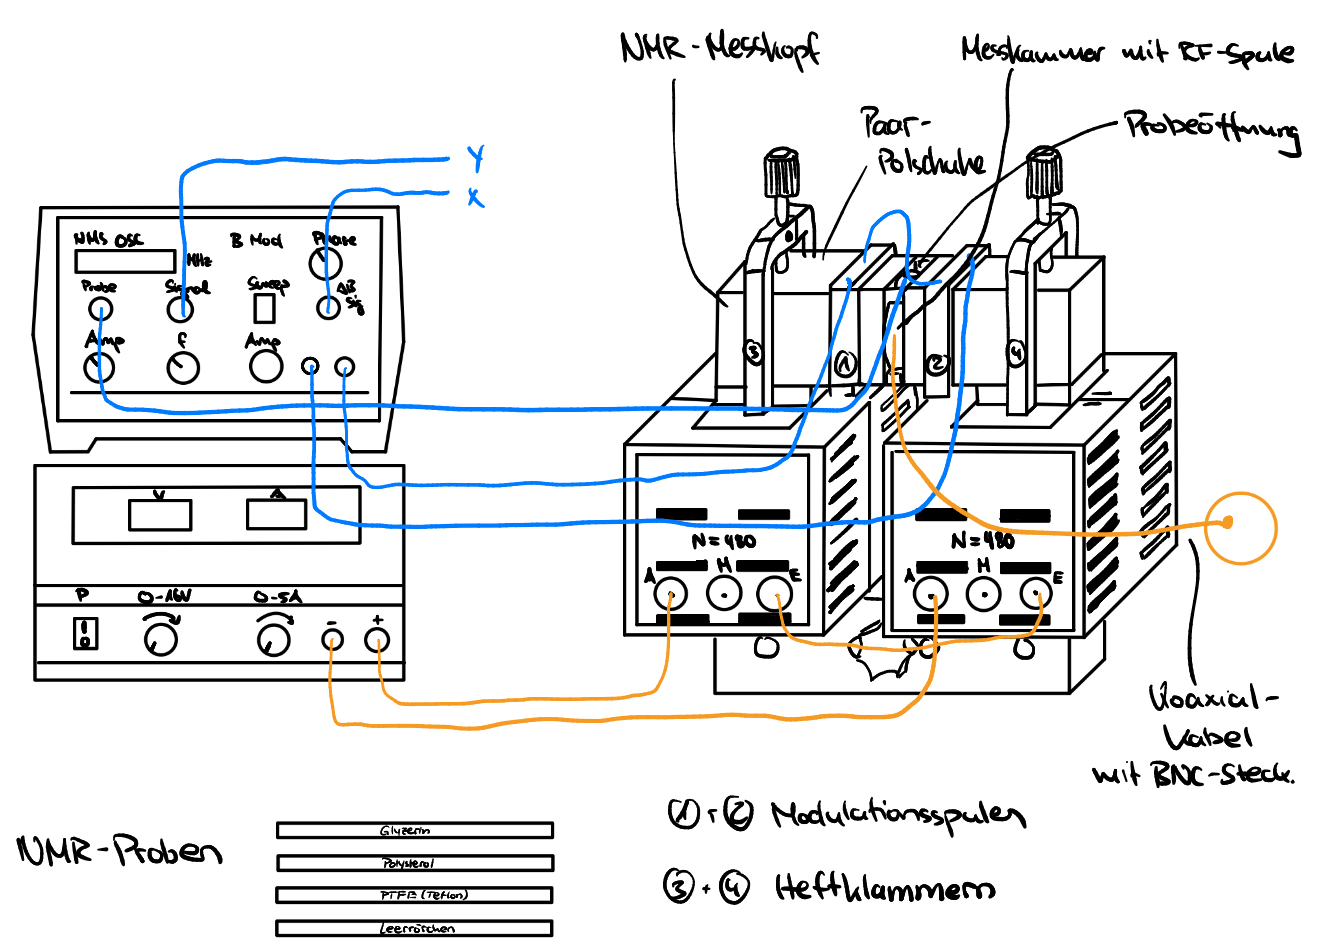
\includegraphics[width=0.7\linewidth]{Abbildungen/TV1-5.jpeg}
        \caption{Versuchsskizze Teilversuch 3}
        \end{figure}

    \item Planung der Durchführung
        \begin{itemize}
           \item Zunächst die PTFE-Probe verwenden
           \item Nachdem Resonanz gefunden wurde, durchführen einer Kalibrierung der x-Achse des Ozilloskops (auf MHz)
           \item Verschieben des Peaks der Resonanz durch Verändern der Frequenz (dabei soll der volle Skalenteil auf dem Bildschirm sein); Frequenz notieren
           \item Anschließend Peak zu einem anderen Skalenteil verschieben und Frequenz notieren
           \item Dadurch Kalibirierung der x-Ablenkung in MHz/Div durchführbar
           \item Vermessen die FWHM in Einheiten des Ozilloskopschirms
           \item Berechnen von der FWHM in Einheiten der Frequenz
           \item Wiederholen der MEssung für Glyzerin, Wasser und Polysyrol (Ausruck für TV1 verwenden)
        \end{itemize}

    \item Vorüberlegungen zur Durchführung \& Auswertung
        \begin{itemize}
            \item Ergebnisse der einzelnen Materialien vergleichen
            \item Unsicherheiten nicht vergessen
        \end{itemize}
        
\end{enumerate}


\newpage

\subsection{Teilversuch 4: Anwendungen in der Chemie (NMR-Skektroskopie)}
\begin{enumerate}[label = (\Roman*)]
    \item Ziel: Wasserstoffgehalt unterschiedlicher Proben bestimmen
    
    \item Versuchsmethode: Durch Referenzmessungen mit bekannten Proben Bestandteile in einer Creme herausfinden
    
    \item Versuchsskizze:
    
        \begin{figure}[H]
        \centering
        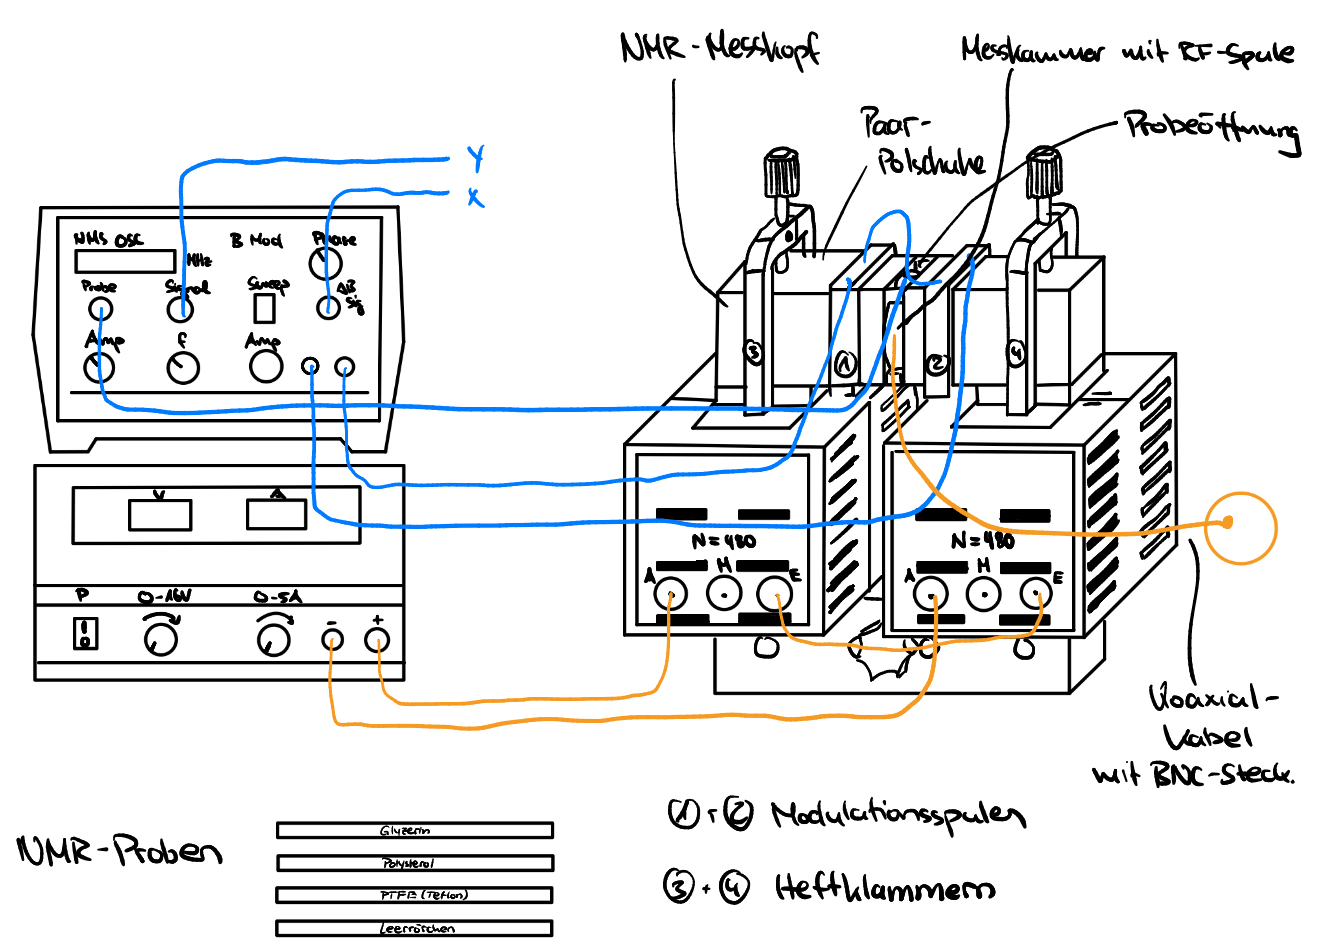
\includegraphics[width=0.7\linewidth]{Abbildungen/TV1-5.jpeg}
        \caption{Versuchsskizze Teilversuch 4}
        \end{figure}

    \item Planung der Durchführung
        \begin{itemize}
           \item Ein Proberörchen mit Creme füllen und Probe in Messkammer positionieren
           \item Resonanzsignal suchen
           \item Aussage über Bestandteile der Probe treffen (Materialien aus TV1 verwenden und vergleichen)
           \item Ergebnis ausdrucken und Messwerte notieren
        \end{itemize}

    \item Vorüberlegungen zur Durchführung \& Auswertung
        \begin{itemize}
            \item Rörchen vor Verscuh gründlich reinigen, damit nur Creme gemessen wird
            \item Zu untersuchende Probe muss genau in Mitte der Messkammer sein
        \end{itemize}
        
\end{enumerate}


\newpage

\subsection{Teilversuch 5: Bestimmung des $g$-Faktors}
\begin{enumerate}[label = (\Roman*)]
    \item Ziel: Bestimmen des $g$-Faktors
    
    \item Versuchsmethode: Der $g$-Faktor für Wasserstoffkerne und Fluorkerne wird mit Hilfe der Kernspinresonanz und eines Teslameters bestimmt
    
    \item Versuchsskizze:
    
        \begin{figure}[H]
        \centering
        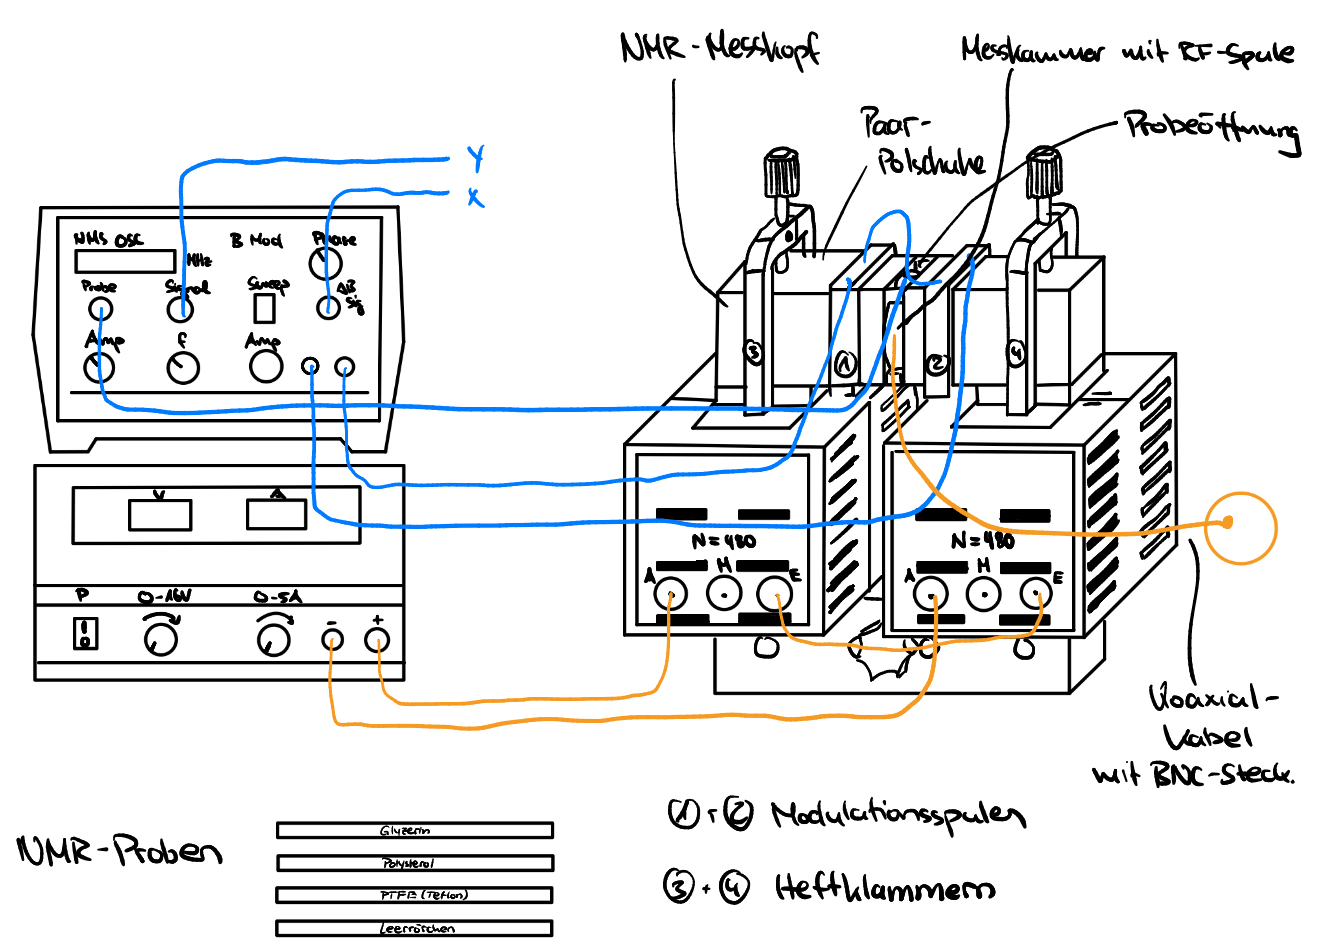
\includegraphics[width=0.7\linewidth]{Abbildungen/TV1-5.jpeg}
        \caption{Versuchsskizze Teilversuch 5}
        \end{figure}

    \item Planung der Durchführung
        \begin{itemize}
           \item Magnetische FLussdichte im Inneren der Messkammer mit B-Feld-Sonde bestimme (maximal gemessenen Wert notieren)
           \item Sonde mit Stativ fixieren und Magnetfeld tangential zur Messkammer an der Stelle mit maximalem Wert messen
           \item Kalibrieren des tangentialen Messpunkts
           \item Einsetzen der Glyzerin-Probe
           \item Frequenzen für verschiedene Frequenzen des RF-Oszillators einstellen, die für Resonanz notwending sind
           \item Jeweiligen Werte des Teslametees notieren
           \item Messung wiederholen für Wasser und Teflon
        \end{itemize}

    \item Vorüberlegungen zur Durchführung \& Auswertung
        \begin{itemize}
            \item Kalibrierfeaktor berechnen und mit Messwerten das Feld im Inneren der Kammer bestimmen
            \item Diagramm erstellen und $g$-Faktoren bestimmen
            \item Mit Literaturwerten vergleichen
        \end{itemize}
        
\end{enumerate}


\newpage

\subsection{Teilversuch 6: Modellversuch zum Spin}
\begin{enumerate}[label = (\Roman*)]
    \item Ziel: Spinflip erzeugen
    
    \item Versuchsmethode: Analogie zwischen Spin und Kreisel anhand eines Kugelkreisels demonstrieren
    
    \item Versuchsskizze:
    
        \begin{figure}[H]
        \centering
        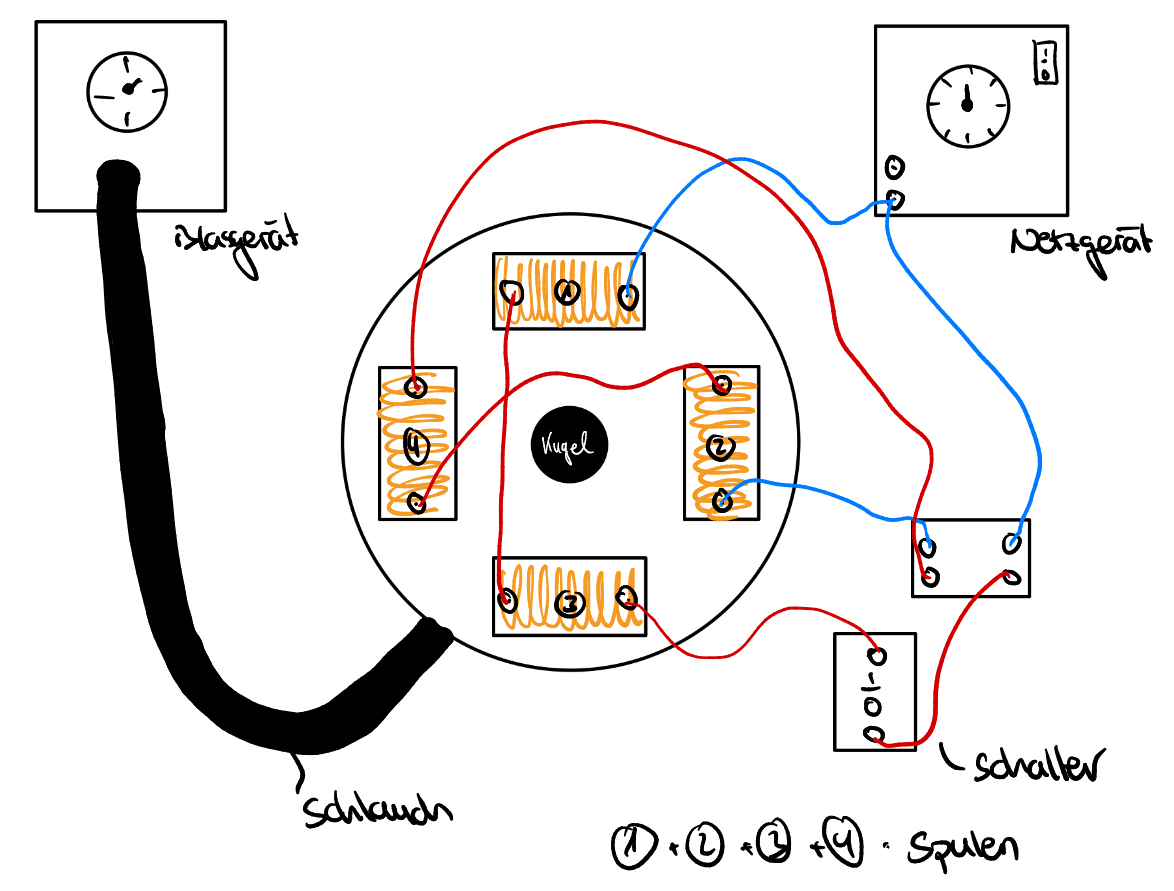
\includegraphics[width=0.7\linewidth]{Abbildungen/TV6.jpeg}
        \caption{Versuchsskizze Teilversuch 6}
        \end{figure}

    \item Planung der Durchführung
        \begin{itemize}
           \item Modellversuch zum Spin
           \item Durch geschicktes Umpolen von Magnetfeld Spinflip erzeugen
           \item Beobachtungen notieren
        \end{itemize}

    \item Vorüberlegungen zur Durchführung \& Auswertung
        \begin{itemize}
            \item Beobachtungen analysieren und beschreiben
        \end{itemize}
        
\end{enumerate}

\newpage

\section{Versuchsprotokoll}

Auf den folgenden Seiten befindet sich das eingescannte Versuchsprotokoll.
Alle Daten wurden selbst gemessen. Sofern fremde Hilfe benutzt wurde,
wurde sie klar gekennzeichnet.

Messunsicherheiten wurden angegeben und folgend in der Auswertung verwendet.
Alle weiteren Rechnungen und Analysen finden in der Versuchsasuwertung statt.

\includepdf[pages={1-18}, pagecommand={\thispagestyle{scrheadings}}, frame=true]{Protokoll.pdf}

\newpage

\section{Auswertung}

\subsection{Teilversuch 1: NMR an flüssigen und festen Proben mit Protonen}

Vergleicht man die Graphen der unterschiedlichen Proben miteinander so fällt auf, dass die Peaks unterschiedliche Ausschläge haben. Diese sind in folgender Skizze eingezeichnet:

    \begin{figure}[H]
        \centering
        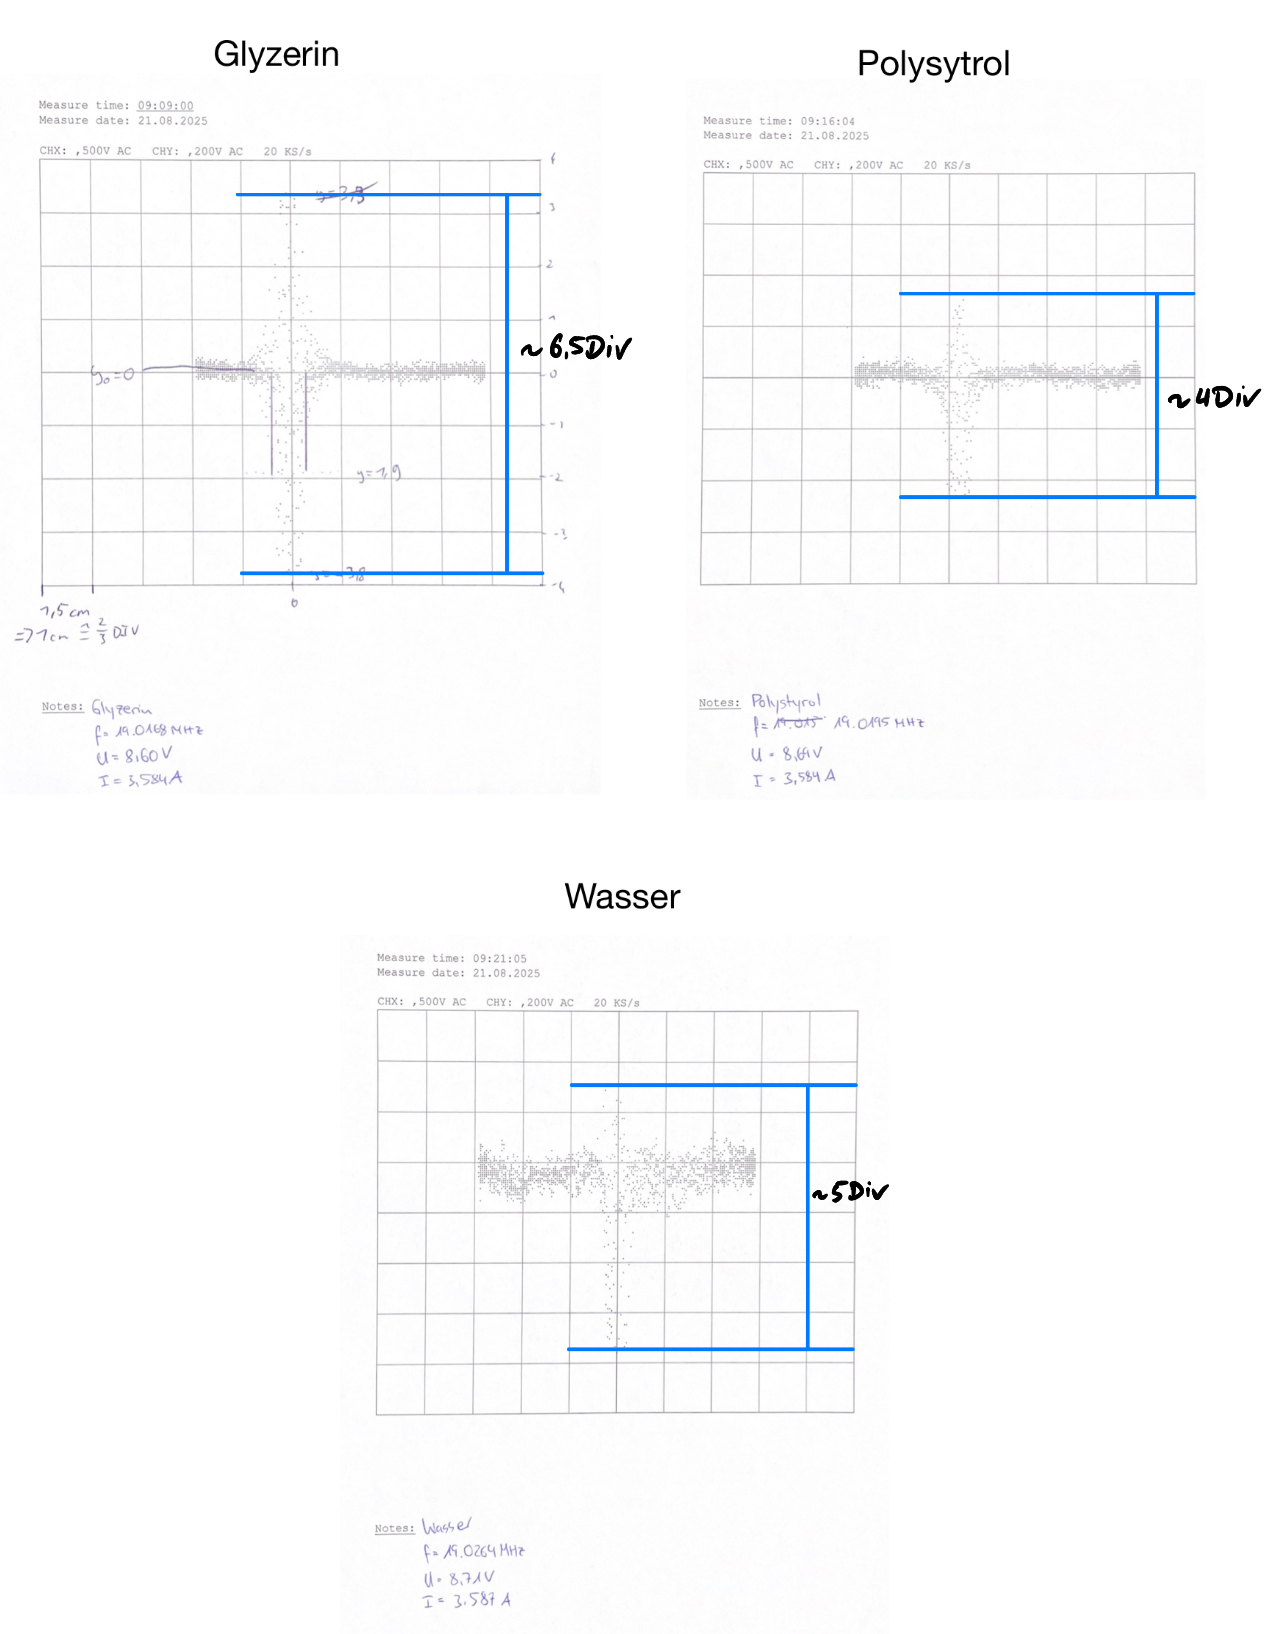
\includegraphics[width=0.7\linewidth]{Abbildungen/VergleichGraphenTV1.jpeg}
        \caption{Vergleich der Resonnzkurven aus Teilversuch 1}
    \end{figure}

Der größte Peak ist bei Glycerin zu beobachtem, dann bei Wasser und der kleinste Peak bei Polystyrol. Die unterschiedlichen Peaks lassen sich durch die unterschiedlichen Protonendichten erklären. Eine höhere Protonendichte führt dabei zu einem stärkeren Signal, was sich in einem größen Peak widerspiegelt. Zudem geht eine höhere Protonendichte immer mit mehr Wassermolekülen, oder anderen protonenhaltigen Vrebindungen, einher (führt zu einem stärkeren Signal). 

Als lässt sich also folgern, dass Glyzerin die größte Protonendichte hat, gefolgt von Wasser und Polystyrol. Polystyrol ist im Vergleich zu den anderen beiden ein Festkörper, was zusätzlich eine schlechtere Beweglichkeit der Spins zur Folge hat.

Anwendung findet dieser Effekt in der Medizin. Hier spielt das Protonendichte-gewichtete MRT eine elementare Rolle, bei welchem Gewebe mit hoher Protonendichte heller erscheint, als andere. \cite{doc}

Desweiteren lässt sich festellen, dass die Breite der unterschiedlichen Peaks nahezu indentisch ist. Die Relaxationszeiten der unterschiedlichen Stoffe, Proben, sind also nahezu identisch. Nahezu identisch sind auch die Resonanzfrequenzen: 
\begin{enumerate}
    \item Resonanzfrequenz Gylcerin: $f_G= \qty{19.0168}{MHz}$
    \item Resonanzfrequenz Polystyrol: $f_P=\qty{19.0195}{MHz}$
    \item Resonanzfrequenz Wasser: $f_W=\qty{19.0264}{MHz}$
\end{enumerate}
Daraus lässt sich darauf schließen, dass die Resonanzfrequenz nur vom angelegten Magnetfeld und der Kernart abhängt. Aus diesem Grund sollte man auch bis Teilversuch 5 das Magnetfeld nicht mehr verändern, um ähnliche Zustände zu ermöglichen.

Auch wenn die Spektren auf den ersten Blick sehr ähnlich wirken, unterscheiden sich diese, wie ersichtlich, in einigen Details, wodurch man viele Rückschlüsse ziehen kann, vor allem auch in der Medizin (MRT - Früherkennung von Krebs). NMR spielt also eine neben der Physik auch in der Medizin eine wichtige Rolle. 

\newpage

\subsection{Teilversuch 2: NMR an einer festen Probe mit Fluorkernen}

Vergleicht man nun die Resonanzkurve von Teflon mit den Resonanzkurven aus Teilversuch 1, so lässt sich als erste Beobachtung festhalten, dass die Resonanzkurve von Teflon lediglich einen Peak in negative y-Richtung hat.

    \begin{figure}[H]
        \centering
        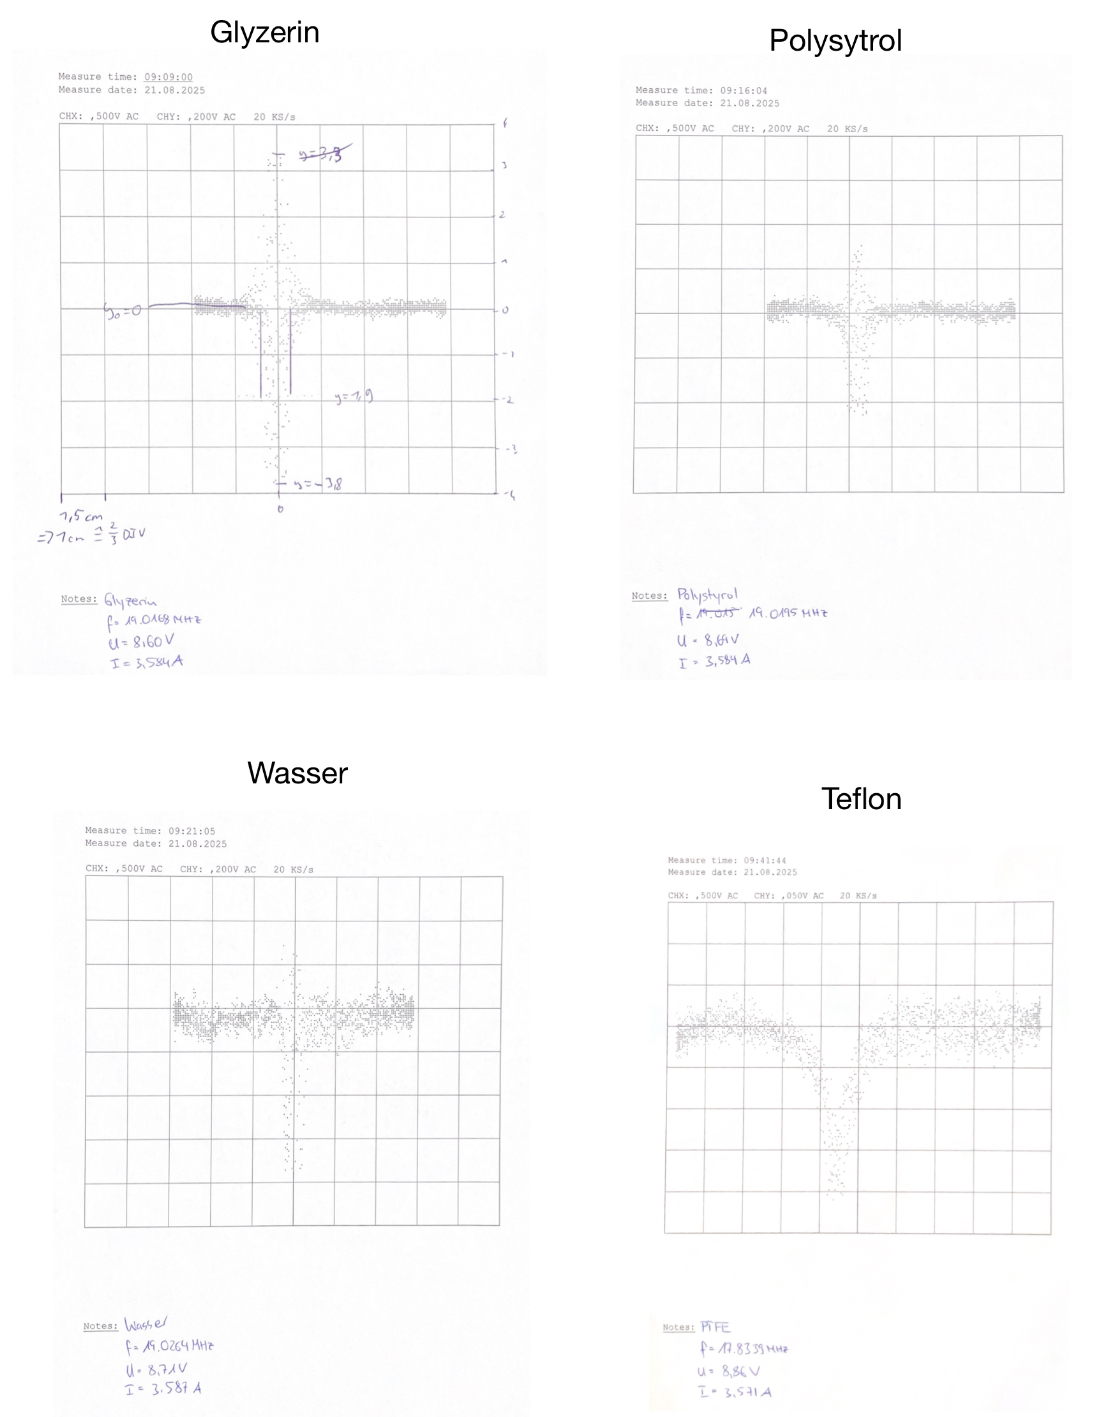
\includegraphics[width=0.7\linewidth]{Abbildungen/VergleichGraphenTV2.jpeg}
        \caption{Vergleich der Resonnzkurve von Teflon mit den Resonanzkurven aus Teilversuch 1}
    \end{figure}

Dieser Effekt tritt auf, da PTFE keine Protonen besitzt, sondern Fluor-Atome. Diese verhalten sich, wie ersichtlich anders als Protonen. Es reagieren also lediglich die Fluorkerne.

Zudem war die Resonazfrequenz von PTFE deutlich geringer als beispielsweise die Resonanzfrequenz von Wasser $f_\text{PTFE} = \qty{17.8339}{MHz} < f_W$. Dies lässt sich durch die Eigenschaft der Fluorkerne erklären, da diese eine starke Elektronegativität aufweisen. 

Die Fluor-Kernspinresonanzspektroskopie hat sich zudem als spektroskopische Methode entwickelt, um fluorierte Verbindungen zu analysieren. Wie uns auch während des Versuchs ersichtlich wurde, war das Resonanzspektrum sehr empfindlich auf Veränderungen. Dadruch erreicht man eine starke Aussagekraft über die chemische Verschiebungen, wodurch sich viele Aussagen über die chemische Umgebung von Fluor treffen lassen. Medizin und Chemie greifen hierauf gerne zurück. \cite{ww}

\newpage

\subsection{Teilversuch 3: Bestimmung der Resonanzbreite}

Die Halbwertsbreiten wurden bereits im Protokoll berechnet, jedoch ohne Unsicherheiten. 
Im Folgenden werden jedoch alle Werte nochmal mit Python, inklusive der Unsicherheiten
berechnet. Die händisch berechneten Werte sind im Protkoll
unter Teilversuch 3 einzusehen.

Um die Halbwertsbreite der Resonanzpeaks zu bestimmen, muss zunächst
die Skalierung der x-Achse des Oszilloskops gefunden werden.
Dies wurde durch eine Verschiebung des Resonanzpeaks von PTFE durchgeführt.
6 divisions (Divs) am Oszilloskop entsprachen einer Frequenzdifferenz
von $\Delta f = \qty{26.3}{kHz}$. Bei einer Skalierung von \qty{500}{mV / Div}
entspricht dies einem Umrechungsfaktor von
$s = \qty{2.192 \pm 0.029}{\kilo\hertz\per Div}$ (\coderef{tv3}).
Mit diesem Faktor können die vom Oszilloskop abgelesenen
Halbwertsbreiten in Frequenzen umgerechnet werden. Dafür ergeben sich folgende Werte:

\begin{table}[H]
    \centering
    \begin{tabular}{c|ccc}
        Probe & Halbwertsbreite [Div] & Osz. Skala [\unit{mV / Div}]
        & Halbwertsberite [\unit{kHz}] \\
        \hline
        PTFE & \num{1.75 \pm 0.05} & \num{500} & \num{7.67 \pm 0.25} \\
        Glycerin & \num{0.70 \pm 0.05} & \num{500} & \num{3.07 \pm 0.23} \\
        Posystyrol & \num{1.00 \pm 0.05} & \num{100} & \num{0.88 \pm 0.05} \\
        Wasser & \num{1.60 \pm 0.05} & \num{100} & \num{1.40 \pm 0.05}
    \end{tabular}
    \caption{Halbwertsbreiten der Resonanzpeaks der vier untersuchten Substanzen
    (\coderef{tv3})}
    \label{table_tv3}
\end{table}

An dieser Stelle ist anzumerken, dass für die Berechnungen vor Ort ein falscher
Umrechnungsfaktor verwendet wurde und sich deswegen diese Ergebnisse von den
vor Ort berechneten unterscheiden.
Für PTFE und Glycerin ist die Unsicherheit um einiges kleiner als für
Polystyrol und Wasser, weil für die letzten beiden eine größerer Zoom am Oszilloskop
gewählt wurde, wodurch die Divisions feiner wurden und somit die absolute Unsicherheit
(welche immer $1 / 20$ Div beträgt), kleiner.

Für die Vermessung der FWHM wurde jeweils nur der untere Peak des Resonanzspektrums
verwendet, weil dieser Peak mehr gaußförmig war als der obere.
Insgesamt war der obere Peak meist etwas breiter als der untere. Hätte man
die Halbwertsbreite also an diesem vermessen, wären vermutlich größere
Werte herausgekommen.

Beim Vergleich der Werte untereinander fällt auf, dass PTFE mit Abstand die größte
Halbwertsbreite hat. Das liegt wahrscheinlich daran, dass bei PTFE die Flourkerne
für die Resonanz sind, während es bei den anderen drei Proben die Wasserstoffkerne
sind. Aufgrund von unterschiedlichen Eigenschaften dieser Kerne, der Atome
und eventuell auch der chemischen Eigenschaften zeigen sie hier ein unterschiedliches
Verhalten. Auch die drei wasserstoffbasierten Substanzen unterscheiden sich
ziemlich stark in ihren Halbwertsbreiten. Hier könnten ebenfalls die verschiedenen
chemischen Eigenschaften der Moleküle bzw. die verschiedenen chemischen
Umgebungen der Wasserstoffatome verantwortlich sein.


\newpage

\subsection{Teilversuch 4: Anwendungen in der Chemie (NMR-Spektroskopie)}

Vergleicht man den Garphen aus Teilversuch 4 (Handcreme) mit den Graphen aus Teilversuch 1, so kann man die Inhaltsstoffe der Handcreme analysieren. Untenstehend wird der Graph der Handcreme nochmal mit den Graphen aus Teilversuch 1 aufgeführt:

    \begin{figure}[H]
        \centering
        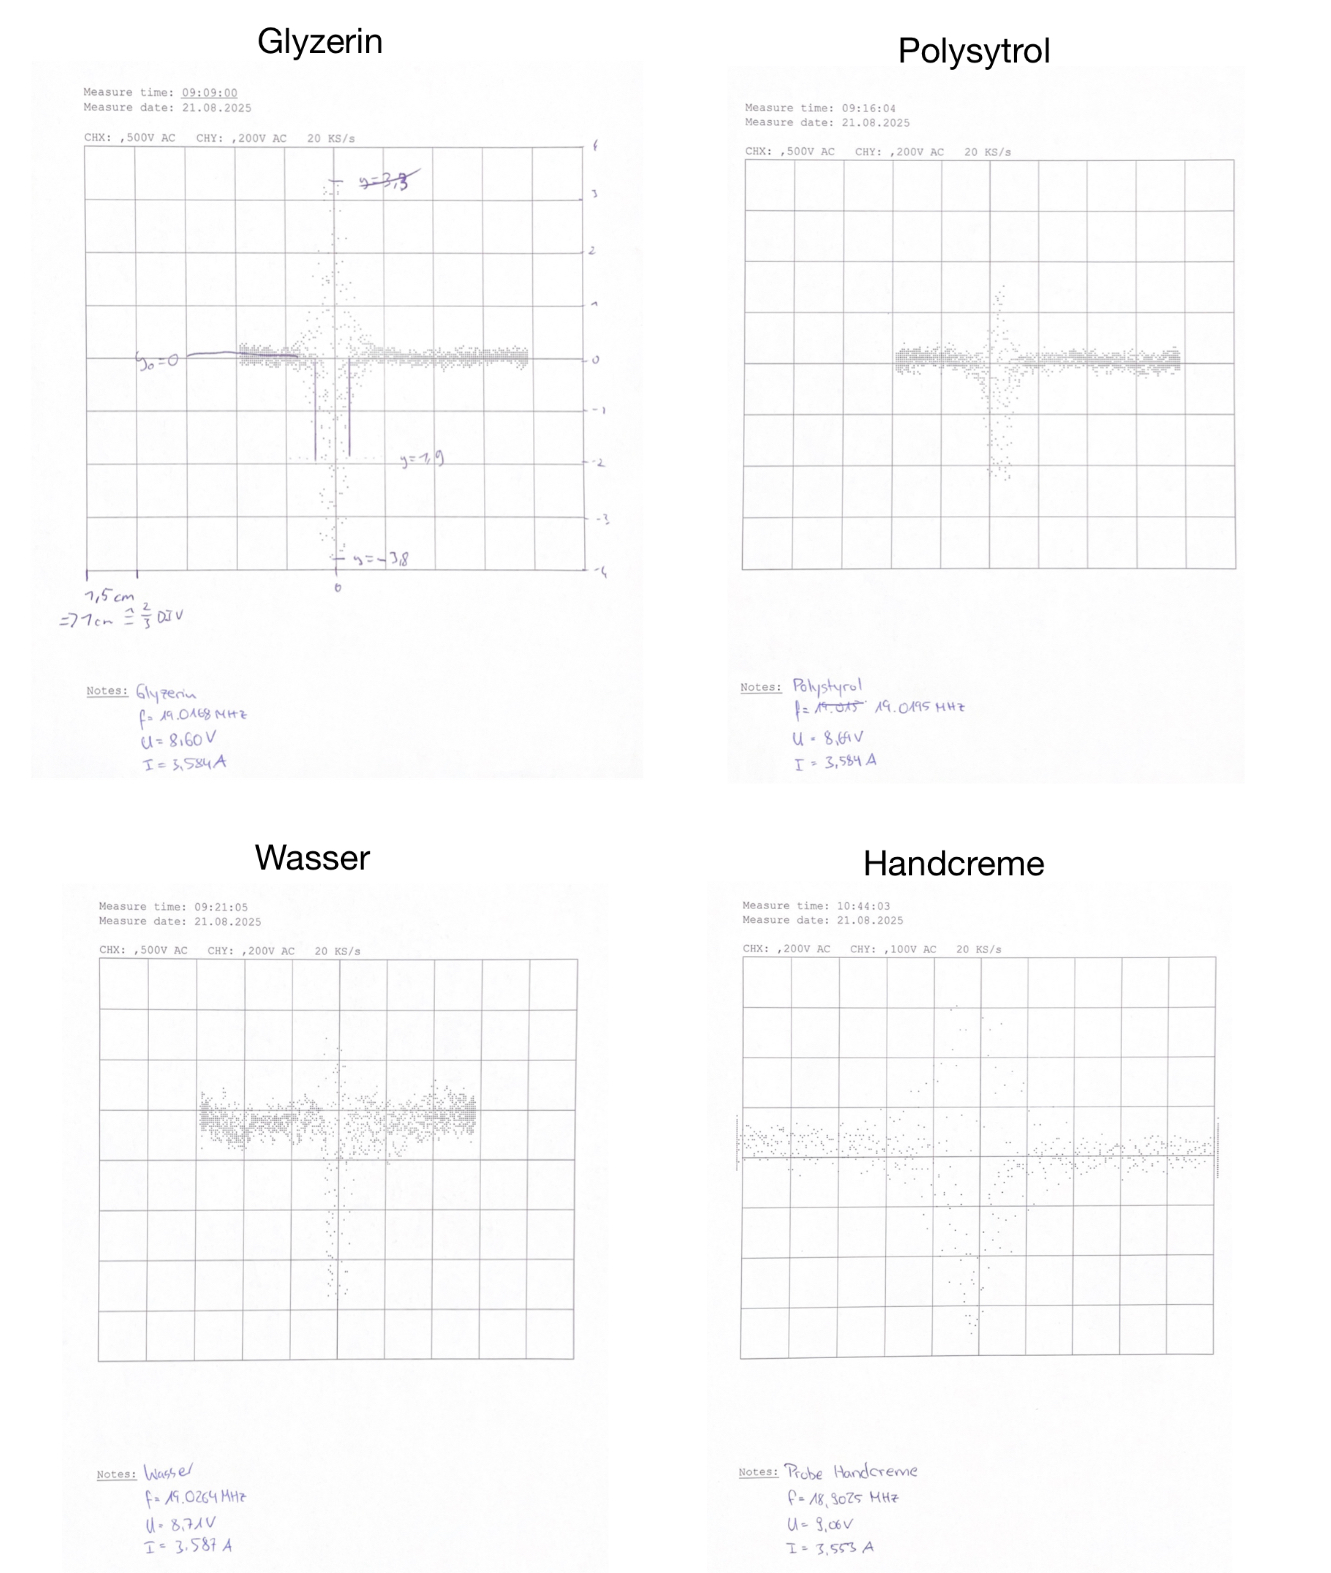
\includegraphics[width=0.7\linewidth]{Abbildungen/VergleichGraphenTV4.jpeg}
        \caption{Vergleich des Graphen der Handcreme mit den Graphen der Proben aus Teilversuch 1}
    \end{figure}

Betrachtet man nun die Graphen, so lässt sich festellen:
\begin{enumerate}
    \item Ähnlichkeit zum Graphen von Glyzerin; Ausschlag in positive und negative y-Richtung
    \item Ähnlichkeit zum Graphen von Wasser; Ausschlag auch in beide Richtungen, aber Ausschlag in negative y-Richtung ist größer
    \item Auch leichte Ähnlichkeit zum Graphen von Polystyrol. Ist aber sinnlos (Begründung untenstehend)
\end{enumerate}

Aufgrund der Ähnlichkeit der Spektren lässt sich darauf schließen, dass die Handcreme aus den Stoffen Wasser und Glycerin besteht. Recherchiert man zusätzlich im Internet, findet man Heraus, dass Wasser und Glycerin zwei der Hauptbestandteile einer Handcreme sind. Dabei fungiert Wasser als Lösungsmittel für alle anderen Bestandteile. Glycerin wirkt feuchtigkeitsspended und bindet Wasser, damit eine homogene Creme entsteht.

Polystyrol lässt sich in Bezug auf die Sinnhaftigkeit in einer Creme ausschließen. Dieser Stoff ist in einer Handcreme nicht enthalten.

Mittels der Spektren lassen sich also Wasser und Gylcerin als Bestandteile der Handcreme-Probe analysieren, beziehungsweise verifizieren.

\cite{cc}

\newpage

\subsection{Teilversuch 5: Bestimmung des $g$-Faktors}

Zunächst müssen aus den Werten des B-Feldes direkt außerhalb der Spule, die mit der
B-Feld-Sonde gemessen wurden, in die Magnetfeldstärken innerhalb der Spule berechnet
werden. Der Kalibrierungsfaktor $c$ ergibt sich aus der ersten Messung des B-Feldes
innerhalb ($B_\text{innen}$) und außerhalb ($B_\text{außen}$)
der Messkammer (ohne Probe):
\[
    c \wideeq \frac{B_\text{innen}}{B_\text{außen}} \wideeq \num{1.632}
    \quad \coderef{tv5}
\]
Damit kann aus unseren Messwerten ($B_\text{gemessen}$) das tatäschliche
Magnetfeld am Ort der Probe berechnet werden:
\[
    B_0 \wideeq c B_\text{gemessen}
\]

Zwischen der Frequenz der RF-Spule und dem Magnetfeld besteht der Zusammenhang
\[
    \nu \wideeq \frac{g \mu_N}{h} \cdot B_0
\]
Trägt man also die gemessene Frequenz gegen die berechneten Magnetfeldstärken
auf, so liegen die Datenpunkte auf einer Gerade mit Steigung $g \mu_N / h$.
Abbildungen \ref{graph_tv5_glycerin}, \ref{graph_tv5_water} und \ref{graph_tv5_ptfe}
zeigen diese Diagramme für Glycerin, Wasser bzw. Polytetraflourethylen.

\begin{figure}[H]
    \centering
    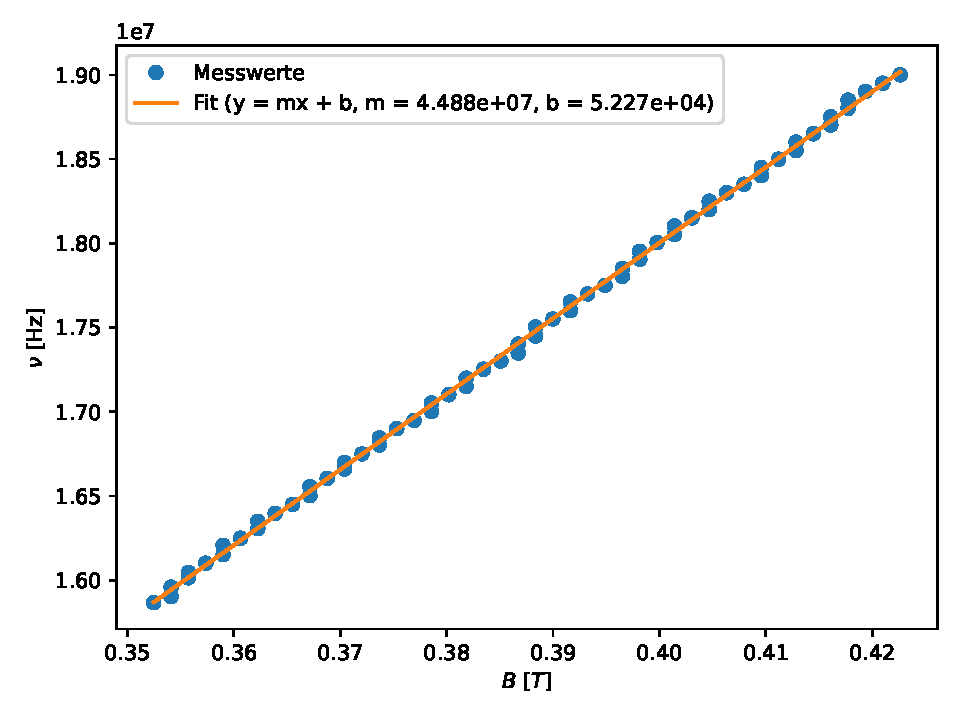
\includegraphics[width=0.7\linewidth]{Abbildungen/Graph_TV5_Glycerin.pdf}
    \caption{$B$-$\nu$-Diagramm für Glycerin (\coderef{tv5})}
    \label{graph_tv5_glycerin}
\end{figure}

\begin{figure}[H]
    \centering
    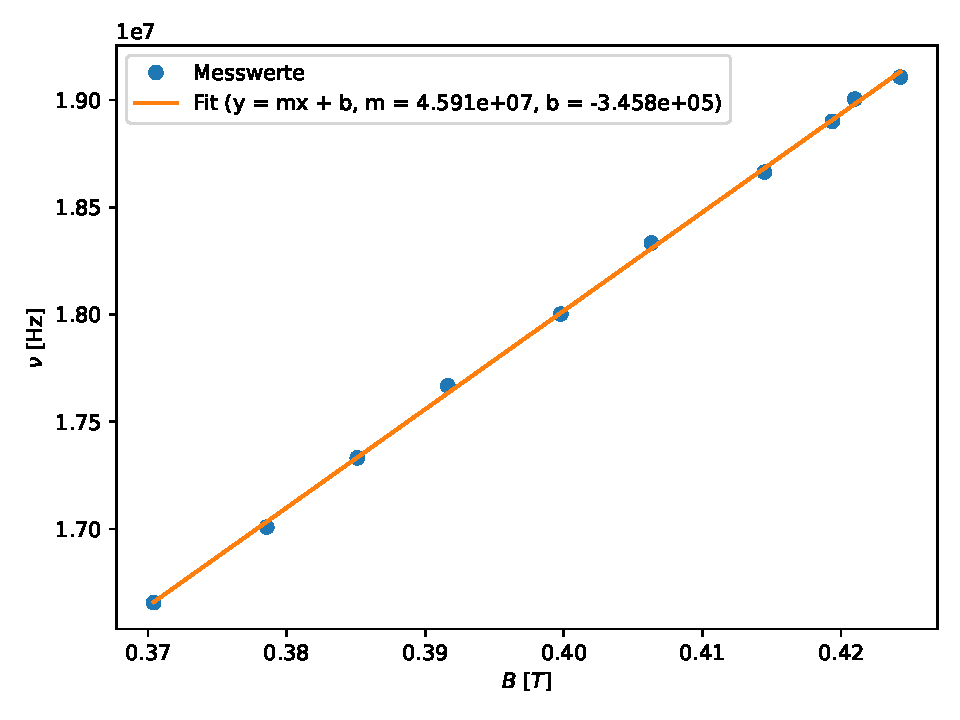
\includegraphics[width=0.7\linewidth]{Abbildungen/Graph_TV5_Wasser.pdf}
    \caption{$B$-$\nu$-Diagramm für Wasser (\coderef{tv5})}
    \label{graph_tv5_water}
\end{figure}

\begin{figure}[H]
    \centering
    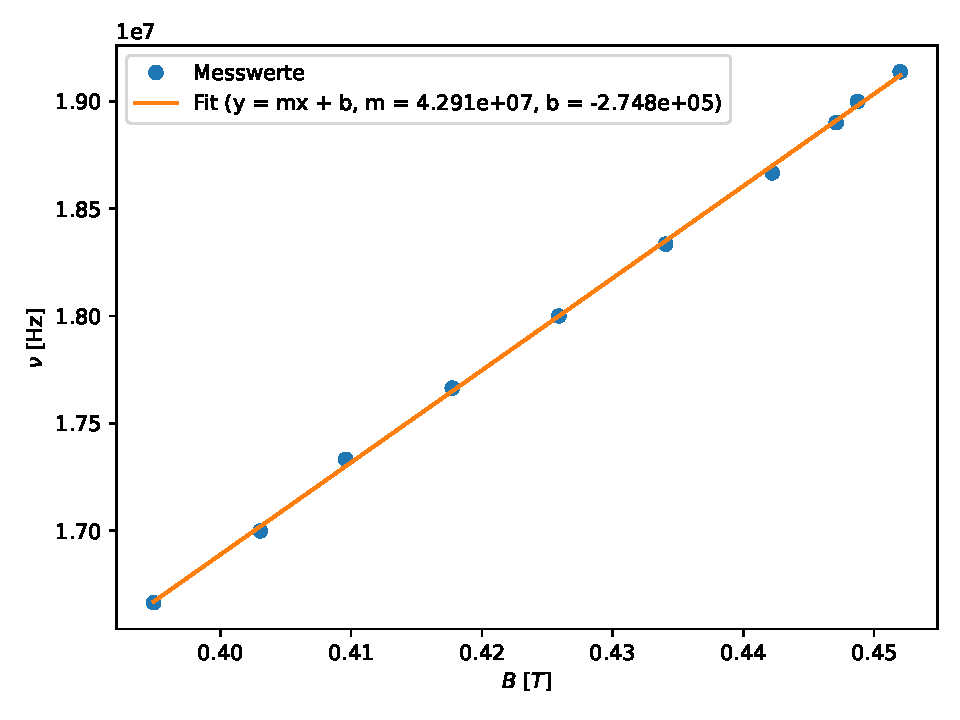
\includegraphics[width=0.7\linewidth]{Abbildungen/Graph_TV5_PTFE.pdf}
    \caption{$B$-$\nu$-Diagramm für Polytetraflourethylen (\coderef{tv5})}
    \label{graph_tv5_ptfe}
\end{figure}

In jeder der drei Messreihen liegen die Punkte schön auf einer Gerade, sodass
die Steigung $m$ der Ausgleichsgerade mit guter Genauigkeit berechnet werden kann.
Daraus kann der jeweilige $g$-Faktor der Probe berechnet werden:
\[
    g \wideeq m \frac{h}{\mu_N}
    \wideeq m \frac{h}{e \hbar / (2 m_p)}
    \wideeq m \frac{4 \pi m_p}{e}
\]

In Tabelle \ref{tabelle_tv5} sind für jede der drei Proben die Werte
der Parameter der Ausgleichsgerade ($m$ und $b$), der daraus berechnete $g$-Faktor
und der Literaturwert für den $g$-Faktor angegeben.
Beim Literaturwert wurde für Glycerin und Wasser der von Wassertoff
($g = 5.5856912$) und für PTFE der von Flour ($g = 5.257723$)
verwendet (Quelle: Skript zur Vorbereitung), weil Glycerin und Wasser
Wasserstoff enthalten, während PTFE kein Wasserstoff, aber dafür Flour enthält.
Zusätzlich ist in der rechten Spalte die Abweichung des experimentell
bestimmten Wertes vom Literaturwert sowohl in Prozent als auch in Vielfachen
der Unsicherheit ($\sigma$) angegeben.

\begin{table}[H]
    \centering
    \begin{tabular}{c|cccc}
        \multirow{2}{*}{Probe}
        & \multicolumn{2}{c}{Fitparameter}
        & \multirow{2}{*}{$g$ (berechnet)}
        % & \multirow{2}{*}{$g$ (Literaturwert)}
        & \multirow{2}{*}{Abweichung} \\
        & $m$ [\unit{\hertz\per\tesla}] & $b$ [\unit{\hertz}] & & \\
        \hline
        Glycerin & \num{4.488 \pm 0.015 e7} & \num{5 \pm 6 e4}
        & \num{5.887 \pm 0.020}
        % & \num{5.5856912}
        & $\qty{5.4}{\percent} \approx \num{15.69} \sigma$ \\
        Wasser & \num{4.59 \pm 4 e7} & \num{-3.458 \pm 0.016 e7}
        & \num{6.02 \pm 0.06}
        % & \num{5.5856912}
        & $\qty{7.8}{\percent} \approx \num{8.50} \sigma$ \\
        PTFE & \num{4.29 \pm 0.04 e7} & \num{-2.7 \pm 1.6 e5}
        & \num{5.63 \pm 0.05}
        & $\qty{7.1}{\percent} \approx \num{7.94} \sigma$
    \end{tabular}
    \caption{Experimentell bestimmte $g$-Faktoren (\coderef{tv5})}
    \label{tabelle_tv5}
\end{table}

Zunächst ist festzustellen, dass die Werte für den $g$-Faktor von Glycerin
und Wasser sehr nahe beieinanderliegen. Das ist zu erwarten, da bei beiden
Substanzen die Kernspinresonanz von den in den Molekülen vorhandenen H-Atomen
kommt. PTFE hat von den drei Substanzen den niedrigsten $g$-Faktor,
was aufgrund des hohen Anteils von Flouratomen in PTFE ebenfalls zu erwarten ist.

Beim Vergleich mit den Literaturwerten fällt jedoch auf, dass unsere experimentell
ermittelten Werte weit von diesen entfernt liegen. Alle drei unterscheiden sich
signifikant von den Literaturwerten.
Insbesondere sind alle drei ermittelten Werte größer als die theoretisch erwarteten.
Dies könnte auf einen systematischen Fehler im Versuchsaufbau oder der Auswertung
hindeuten. Beispielsweise könnte die ursprüngliche Messung des Magnetfeldes
im Inneren der Messkammer zu niedrig gemessen worden sein.
Dadurch würde die Steigung der Ausgleichsgeraden und damit die $g$-Faktoren
zu hoch berechnet werden, was den Fehler (zumindest teilweise) erklären würde.


\newpage

\subsection{Teilversuch 6: Modellversuch zum Spin}

Da bei diesem Versuch nur qualitative Beobachtungen getroffen werden, ist keine Berechnung bei der Auswertung notwendig. Die getroffenen Beobachtungen werden im Folgenden noch einmal beschrieben und physikalisch erklärt. Man konnte beobachten, dass sich die Billiardkugel reibungslos dreht und sich entlang des Magnetfelds ausrichtet. Die Ausrichtungslage der Kugel ist hierbei abhängig von der Schalterstellung und beträgt $\pm\ang{45}$ gegenüber der statischen Spulenpaare. 

Durch geeignetes Umschalten des Magentfeldes war es nun möglich, die Präzessionsamplitude immer weiter zu vergrößern, bis die Kugel schließlich flipt.

Da dies ein Modellversuch ist, entsprechen die einzelnen Komponenten physikalischen Eigenschaften:
\begin{itemize}
    \item Die Richtung der Kugelbewegung beschreibt den eigentlichen Spin
    \item Die Ruhelage der Kugel beschreibt den stabilen Spin-Zustand
    \item Erreicht man schließlich die entgegengesetzte Lage der Kugel entspricht dies dem Spin-Flip
    \item Das magentische Moment des Kerns wird beschrieben durch die Kugel im Spulenfeld
    \item Das Hochfrequenzfeld, welches den Spin flipt wird durch die wechselnden Ströme in den Spulen, welche due Kugel anregen, dargestellt
\end{itemize}

Die Kugel flipt also, da das oszillierende Magnetfeld im Resonanzfall die richtige Menge an Energie zuführt.

Abschließend lässt sich noch festhalten, dass dieser Versuch den Spin nur modellhaft darstellen beziehungsweise veranschaulichen kann und nicht die Realität darstellt, da in Wirklichkeit ein quantisierter Zwei-Stunstand-Flip stattfindet.

\newpage


\section{Anmerkung: Graphische Auswertung und Fehlerfortpflanzung mit Python-Code}

Alle Berechnungen inkl. Fehlerbestimmung wurden mit einem selbstgeschriebenen
Python-Skript durchgeführt, um uns die Arbeit zu erleichtern und Fehler zu
vermeiden. Alle Ergebnisse, die auf diese Weise zustande gekommen sind,
sind entsprechend mit einem \colorbox{codebg}{blauen Hintergrund} gekennzeichnet;
s. folgendes Beispiel:
\[
    F \wideeq ma \wideeq \qty{20}{\kg} \cdot \qty{9.81}{\meter\per\square\second}
    \wideeq \qty{19.6 \pm 0.5}{\newton} \quad \coderef{tv1}
\]
Dies soll bedeuten, dass die Berechnung des Wertes und der Unsicherheit von der
Python-Funktion namens \verb|tv1| durchgeführt wird.
Die Unsicherheit wird - sofern nicht anders angegeben - mithilfe der Gauß'schen
Fehlerfortpflanzung berechnet.
Außerdem wird das Python-Package \texttt{matplotlib} zum Erstellen
von Graphen verwendet.

Der verwendete Code ist sowohl auf GitHub verfügbar (\githuburl) als auch auf den
folgenden Seiten zu finden und kann mit dem Befehl \texttt{python Main.py}
ausgeführt werden. Für eine genauere Beschreibung des Codes siehe die README-Datei
auf GitHub sowie die Kommentare im Code.
(Manche Sonderzeichen im Code (ä, ö, ü, $\Delta$, etc.) werden von \LaTeX nicht
richtig erkannt, deswegen kann der Code auf den nachfolgenden Seiten an einigen
Stellen unvollständig erscheinen. Auf GitHub wird aber alles richtig angezeigt.)

\newpage


\verb|main.py|:
\lstinputlisting[language=Python]{Code/main.py}
\newpage

\verb|expressions.py|:
\lstinputlisting[language=Python]{Code/expressions.py}
\newpage

Output:
\lstinputlisting{Code/output.txt}

\end{document}